\documentclass{article} % For LaTeX2e
\usepackage{theme,times}
\usepackage{hyperref}
\usepackage{url}
\usepackage{graphicx}
\usepackage{amssymb}
\usepackage[fleqn]{amsmath}
\DeclareMathOperator{\E}{\mathbb{E}}
\usepackage{graphicx}
\usepackage{float}
\usepackage{placeins}
\usepackage{subfig}
\usepackage{tikz}
\usepgflibrary{arrows}
\usetikzlibrary{shapes}
\renewcommand{\baselinestretch}{1.2}
\newcommand*\circled[1]{\tikz[baseline=(char.base)]{
            \node[shape=circle,draw,inner sep=2pt] (char) {#1};}}
\usepackage{setspace}
\usepackage[utf8]{inputenc}


\title{Optimization under Fairess Constraints}


\author{}

% The \author macro works with any number of authors. There are two commands
% used to separate the names and addresses of multiple authors: \And and \AND.
%
% Using \And between authors leaves it to \LaTeX{} to determine where to break
% the lines. Using \AND forces a linebreak at that point. So, if \LaTeX{}
% puts 3 of 4 authors names on the first line, and the last on the second
% line, try using \AND instead of \And before the third author name.

\newcommand{\fix}{\marginpar{FIX}}
\newcommand{\new}{\marginpar{NEW}}

%\nipsfinalcopy % Uncomment for camera-ready version

\begin{document}


\maketitle

\begin{abstract}
To solve the problem of discrimination or unfairness treatment in decision making process, this project introduce a new method called fairness constrained optimal decisions. We apply our model in different data type domain with different machine learning algorithms. We also explore the varieties of applications in industry with different utility models. We also analyze the performance of our models with different causal effect constraints which shows a trade-off between causal effect and prediction accuracy or maximized utility.
\end{abstract}
\section{Introduction}
\hspace*{1em}Algorithms from decision making and machine learning are increasingly playing important roles on people's lives, including policing, pricing, hiring, criminal sentencing and so on. However, discrimination may happen during the decision making process. This happens when sensitive attributes information has disparate impacts to the outcomes. Such sensitive attributes usually include gender, religion, physical ability and so on. These are referred as the protected attributes in Federal Laws and regulations. Take criminal sentencing as an example, blacks were more than twice as likely as whites to be labeled risky even though they didn't continue to commit a crime.\\
\hspace*{1em}In this project, we focus on the problem of fairness in decision making process and machine learning algorithms, and we apply the causal fairness principles to balance the outcome with respect to sensitive attributes to decision variables.\\
\hspace*{1em}Our contribution in this project is we apply causal effect measures as constraints in decision making process. And we solve the utility maximization problem in discrete domain and continuous domain where relationship between variables is linear. Another contribution is that we also apply the constraints on classification and regression algorithms. For the classification, we apply the non convex constraints and optimize the model over discrete domain. For the regression, we apply convex optimization over continuous domain.\\
\hspace*{2em}The domain is restricted to a general causal structural model below:\\
\centerline{
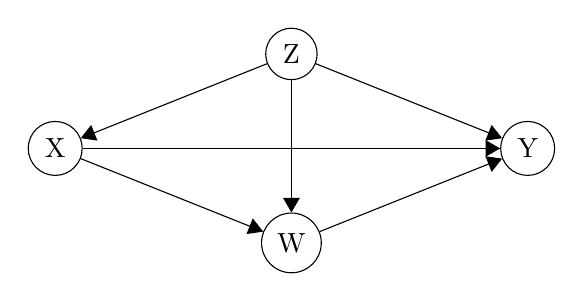
\begin{tikzpicture}
\tikzstyle{every node}=[draw, shape=circle];
   \node (n1) at (0,0) {X};
   \node (n2) at (6,0) {Y};   
   \node(n3) at (3,1.2) {Z};
   \node(n4) at (3,-1.2){W};
  \foreach \from/\to in {n1/n2,n3/n2,n3/n1,n3/n4,n4/n2,n1/n4}
    \draw[-triangle 60] (\from) -- (\to);
\end{tikzpicture}
}
\hspace*{1em}which X stands for the protected attribute, Y for the decision variable, W the mediator and Z an observed background variable.\\
\section{Optimization over Discrete Domain}
\hspace*{1em}Assumption:\\
\hspace*{1em}1. The distribution is in binary domain.\\
\hspace*{1em}2. The distribution of the states is known.\\
\hspace*{1em}3. Specified utility function.\\
\hspace*{1em}4. Action or decision is going to be taken only when the maximize utility is achieved. Higher value of utility corresponds to greater likelihood of Y=1.\\
\hspace*{1em}e.g. In a hiring practice, we are going to take an action of whether or not to hire the person. We have a utility function that evaluates the person's ability in work and the utility function is known. And there is a optimal action of hiring or not hiring when the maximized utility value is achieved.
Decision Formulation:\\
\hspace*{1em}State: X, W, Z\\
\hspace*{1em}Decision variable: Y, if Y=1, take action or make decision. e.g. hiring the person or releasing the criminal.\\
\hspace*{1em}Utility function: U = f(x, w, z, y). Decision is made when maximized utility is achieved under certain state.\\
\hspace*{1em}Objective: Maximize the expected utility\\
\hspace*{1.2em}$\underset{Y}{maximize}\,\,\,\, \E[U]$\\
$= {maximize}\,\,\,\,\sum\limits_{y, x, w, z} P(x, w, z, y)U(x, w, z, y)$\\
$= {maximize}\,\,\,\,\sum\limits_{x, w, z, y} P(Y=y|x, w, z)P(x, w, z)U(x, w, z, y)$\\
Constraints: causal effect with respect to sensitive attribute X and action Y.(DE, IE, SE)\\
\hspace*{5em}$DE =\sum\limits_{z, w}(P(Y|x_1, w, z)-P(Y|x_0, w, z))P(w|x_0, z)P(z|x_0)$\\
\hspace*{5em}$IE =\sum\limits_{z, w}P(Y|x_0, w, z)(P(w|x_1,z)-P(w|x_0, z))P(z|x_1)$\\
\hspace*{5em}$SE =\sum\limits_{z, w}P(Y|x_0, w, z)P(w|x_0, z)(P(z|x_1)-P(z|x_0))$\\
\hspace*{1em}Formulation of linear programming:\\
\hspace*{1em}Let $p_{i, jkl}$ denotes $P(Y=i |X=j, W=k, Z=l)$, e.g. $p_{1,000}$ represents $P(Y=1 |X=0, W=0, Z=0)$.\\
The whole problem can be rewritten as:\\
\hspace*{7em}{$ \underset{p_{i, jkl}}{maximize}\,\,\,\,\sum_{i=0}^{1} \sum_{j=0}^{1}\sum_{k=0}^{1}\sum_{l=0}^{1}p_{i, jkl}P_{x_jw_kz_l}U(x_j, w_k, z_l, y_i) $ \hfill (1)}\\
\hspace*{9em}{s. t. $\sum_{i=0}^{1} p_{i, jkl} = 1, \forall j, k, l$}\\
\hspace*{11.3em}{$0\leq p_{i, jkl} \leq 1, \forall i, j, k, l$}\\
\hspace*{11.3em}{$|\sum_{k=0}^{1}\sum_{l=0}^{1} (p_{1, 1kl}- p_{1, 0kl}) P_{w_k|x_0z_l}P_{z_l|x_0}| \leq c_1$, (constrained on DE)}\\
\hspace*{1em}In the above equation, the big P denotes the conditional distribution regrading X, Z, W which is assumed to be given. The small p denotes the conditional distribution regrading Y which is the objective.\\
\hspace*{1em}Constraints can also be set in the following ways:\\
\hspace*{1em}Constrained on DE+IE: \\
\centerline{$|\sum_{k=0}^{1}\sum_{l=0}^{1} (p_{1, 1kl}- p_{1, 0kl}) P_{w_k|x_0z_l}P_{z_l|x_0} + \sum_{k=0}^{1}\sum_{l=0}^{1} p_{1, 0kl}(P_{w_k|x_1z_l}- P_{w_k|x_0z_l})P_{z_l|x_1}| \leq c_2$}
Constrained on total variation: \\
\centerline{$|\sum_{k=0}^{1}\sum_{l=0}^{1} (p_{1, 1kl}- p_{1, 0kl}) P_{w_k|x_0z_l}P_{z_l|x_0} + \sum_{k=0}^{1}\sum_{l=0}^{1} p_{1, 0kl}(P_{w_k|x_1z_l}- P_{w_k|x_0z_l})P_{z_l|x_1} + $}
\centerline{$\sum_{k=0}^{1}\sum_{l=0}^{1} p_{1, 0kl}P_{w_k|x_0z_l}(P_{z_l|x_1}-P_{z_l|x_0})| \leq c_3$}
\hspace*{1em}The optimization problem (1) is a linear program in variables respect to CPDs conditioning on states:  (1)The objective function is a linear function of these parameters. (2)The constraints are linear or convex which specify the optimal solution in a convex hull.\\
\hspace*{1em}And we can say that the value of Y can be defined when the conditional probability of y given X, Z,W is greater than some threshold.\\

\section{Optimization over Continuous Domain}
\hspace*{1em}Assumption:\\
\hspace*{1em}1. Suppose the causal relationship is linear between variables.\\
\hspace*{1em}2. Decision variables are continuous random variables, and take any value between the lower bound and upper bound. e.g. $d\in (\underline{d}, \overline{d})$\\
\hspace*{1em}3. Decision is made when utility maximization is achieved. e.g. the maximized reward or revenue.\\
\hspace*{1em}4. Utility function is deterministic and known.\\
\hspace*{1em}5. The utility function is continuous and differentiable.\\
\subsection{Linear Utility}
\hspace*{1em}The constraints are linear:\\
\hspace*{5em}DE:  $DE_{x_0,x_1}(Y) = \beta_{xy}$,\\
\hspace*{5em}IE: $IE_{x_0,x_1}(Y) = \beta_{wy}\beta_{xw}$,\hfill(2)\\
\hspace*{5em}SE: $SE_{x_0,x_1}(Y) = (\beta_{zy}+\beta_{zw}\beta_{wy})\beta_{xz}$,\\
\hspace*{1em}where $\beta$ represent the corresponding regression coefficient.\\
Hence, Y can be represented by linear regression: $Y = \beta_{xy}X+\beta_{wy}W+\beta_{zy}Z + \beta_0.$\\
$\beta = [\beta_{xy}, \beta_{wy}, \beta_{zy}, \beta_0]^T$\\
Objective function: $\underset{Y}{maximize}\,\,\,\, \E[U(Y)]=\underset{\beta}{maximize}\,\,\,\, \E[U(\beta)]$\\
The whole problem is a linear program:\\
\hspace*{12em}$ \underset{\beta}{maximize}\,\,\,\, \E[U(\beta)] \hfill (3)$\\
\hspace*{10em}{s. t. $\underline{y}\leq A^T\beta \leq \overline{y}$}\\
\hspace*{15em}{$|\beta_{xy}| \leq c_1$ \hfill(constrained on DE)}\\
\hspace*{1em}Simplex method can be applied to solve this problem easily.\\
\subsection{Nonlinear Utility}
\subsubsection{Concave Utility}
\hspace*{1em}Since the utility function is a differentiable convex function in the feasible region and the constrained region is a convex hull, then the KKT optimality conditions are sufficient for the global optimality of a feasible solution. 
\subsubsection{Non-concave Utility}
\hspace*{1em}Generally, arbitrary nonconcave or nonconvex optimization problems are not easy to solve. However, since we've restricted the domain in a linear causal model, the whole problem becomes into linear constrained nonlinear optimization problem.\\
\hspace*{1em}Let $|A^T\beta|\leq c$ denotes the linear fairness constraints. It could be any combination of DE, SE and IE. The constraints are all continuous and differentiable over $R^n$.\\
\hspace*{1em}Assume the utility function is determinstic. Hence, the general problem is:\\
\hspace*{12em}$\underset{\beta}{maximize}\,\,\,\, f(\beta), s.t. |A^T\beta|\leq c$ \hfill(4)\\ 
\hspace*{1em}Let g($\beta$) denotes the constrain as: g($\beta)\leq 0$, g($\beta$) is continuous over $\beta$.\\
\hspace*{1em}Sometimes the global optimal solution can be found if the nonconcave utility function has special structures:\\
\hspace*{1em}\textbf{1. Monotonic Utility}\\
\hspace*{1em}Monotonicity optimization problems are a very important part in economic and communication networks.\\
\hspace*{1em}For linear constraints: g($\beta_1, ... \beta_n$) is monotone in $\beta_i$, for $\forall$ i=1, 2, ... n\\
\hspace*{1em}According to the monotonicity principles, we can have the following result:\\
\hspace*{1em}Assume $\beta$ has lower bound and upper bound, $\beta\in(\beta^L, \beta^U)$\\
\hspace*{1em}Assume $f$ is monotonic utility function with respect to $\beta$.\\
\hspace*{1em}i) Suppose the constraints $g(\beta)$ are monotone increasing in $\beta$, then there exists a global optimal solution of problem (4) if at least one variable $\beta_k$ in $f$ in not monotone increasing.\\
\hspace*{1em}\textit{Proof}   The proof is very straightforward. Let $\beta^* = (\beta^*_1, \beta^*_2, ..., \beta^*_n)$ denote a global optimum of problem (4). If $f$  is not monotone increasing in $\beta_k$, obtaining the value $\beta_k$ such that function $g(\beta^*_1, \beta^*_2, ..., \beta^*_n)$ becomes equal to zero. And this is always possible since $\beta$ has lower bound.\\
\hspace*{1em}ii) More generally, suppose the constraints $g(\beta)$ are monotone increasing in $\beta_i$, monotone decreasing in $\beta_j$, and independent of $\beta_k$. If $f$ has the different monotonicity with respect to $\beta_i$ and $\beta_j$, and is monotone increasing or decreasing in $\beta_k$, then the constraints are tight and there exists a global optimal solution of problem (4).\\
\hspace*{1em}iii)One special case is the problem to maximize an increasing function subject to an increasing constraint with nonnegative coordinates:\\
\centerline{$max\{f(\beta)| x\in G\},$}
\hspace*{1em}where $G$ is a compact normal set $G:= \{ \beta\in R^n_+|g(\beta)\leq0\}$\\
\hspace*{1em}Suppose $g(\beta)$ is increasing, then a normal set G can be approximated by ployblocks.\\
\hspace*{1em}\textbf{2. Generic Utility}\\
\hspace*{1em}If the function is generic, there are several methods that can be applied:\\
\hspace*{1em}1. Linearly constrained Lagrangian Methods: We assume the utility function is differentiable. LCL methods can solve a sequence of subproblems that maximize an augmented Lagrangian function subject to linear inequality constraints. But sometimes it may not converge from arbitrary starting points. And the optimal solution might not be global optimal.\\
\hspace*{1em}2. Genetic Algorithm: Genetic algorithm can approximate the global optimal point. It depends on the specific problems. Some problems might be effectively solved by genetic algorithm. Sometimes other optimization algorithms may be more efficient that genetic algorithm.\\
\section{Fairness in Machine Learning Algorithm}
\subsection{Fairness in Classification}
\hspace*{1em}Apply the causal fairness measures in logistic regression model:\\
\centerline{$p(y_i=1|x_i, \theta) = \frac{1}{1+e^{-\theta^Tx_i}}$}
\hspace*{1em}Consider the direct causal effect:\\
$DE = (\frac{1}{1+e^{-\theta_x-\theta_z-\theta_w}}- \frac{1}{1+e^{-\theta_z-\theta_w}}) P_{w_1|x_0z_1}P_{z_1|x_0} + $
$(\frac{1}{1+e^{-\theta_x-\theta_z}}- \frac{1}{1+e^{-\theta_z}}) P_{w_0|x_0z_1}P_{z_1|x_0} + $\\
\hspace*{3em}$(\frac{1}{1+e^{-\theta_x-\theta_w}}- \frac{1}{1+e^{-\theta_w}}) P_{w_1|x_0z_0}P_{z_0|x_0} + 
(\frac{1}{1+e^{-\theta_x}}- \frac{1}{2})P_{w_0|x_0z_0}P_{z_0|x_0}$\\
\hspace*{1em}Rewrite the expression in a simpler way:\\
$DE = k_1(\frac{1}{1+e^{-\theta_x-\theta_z-\theta_w}}- \frac{1}{1+e^{-\theta_z-\theta_w}}) + k_2(\frac{1}{1+e^{-\theta_x-\theta_z}}- \frac{1}{1+e^{-\theta_z}}) +$\\
\hspace*{3em}$ k_3(\frac{k_3}{1+e^{-\theta_x-\theta_w}}- \frac{1}{1+e^{-\theta_w}})+k_4(\frac{1}{1+e^{-\theta_x}}- \frac{1}{2}) $\\
\hspace*{1em}The problem becomes into:\\
\hspace*{12em}$\underset{\theta}{minimize} -\sum_{i=1}^{N}\,\,\, logp(y_i=1|x_i, \theta) \hfill(5)$\\
\hspace*{6em}{ subject to $|k_1(\frac{1}{1+e^{-\theta_x-\theta_z-\theta_w}}- \frac{1}{1+e^{-\theta_z-\theta_w}}) + k_2(\frac{1}{1+e^{-\theta_x-\theta_z}}- \frac{1}{1+e^{-\theta_z}}) +$\\
\hspace*{10em}$k_3(\frac{k_3}{1+e^{-\theta_x-\theta_w}}- \frac{1}{1+e^{-\theta_w}})+k_4(\frac{1}{1+e^{-\theta_x}}- \frac{1}{2}) | \leq c_1$, (constrained on DE)}\\
\hspace*{1em}The constraints are not linear and not convex. The problem is a convex objective function with nonlinear constraints.\\
\FloatBarrier
\begin{figure}[!htb]
    \centering
    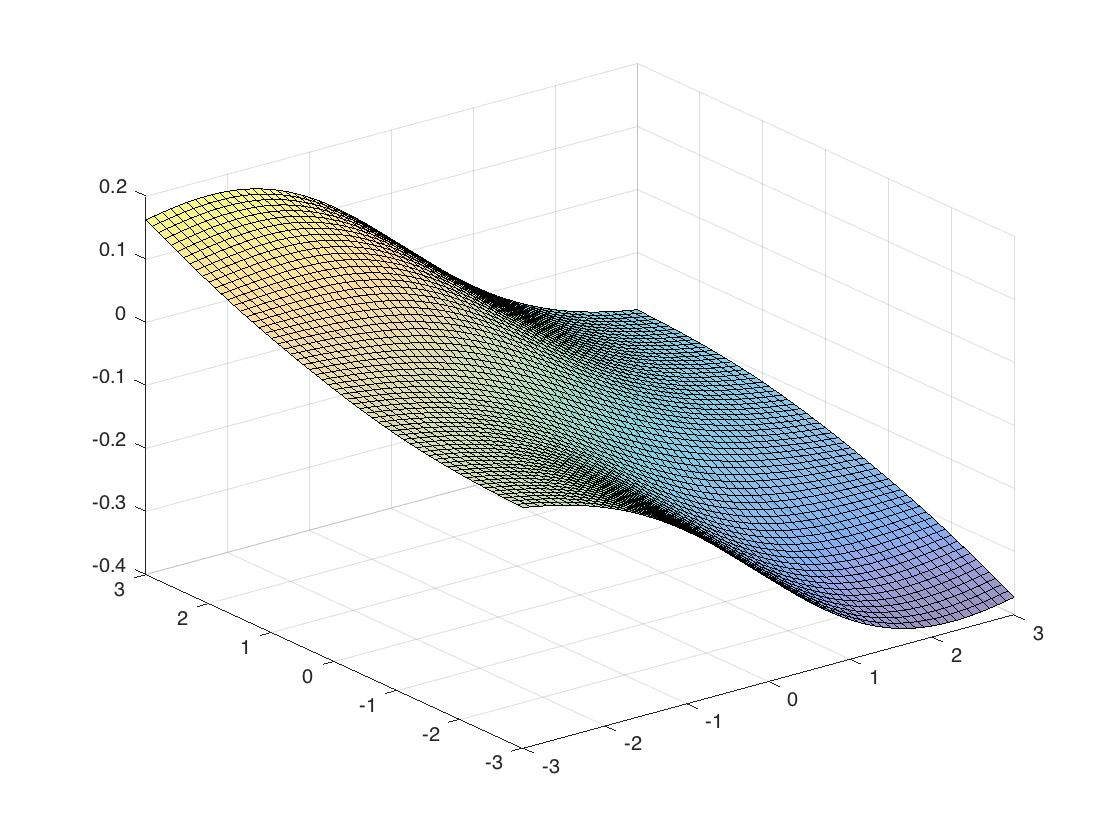
\includegraphics[height=3.5in]{constraints.jpg}
    \caption{non-linear constraint}
\end{figure}
\FloatBarrier
\hspace*{1em}From the above figure, we can see that the constraints are partly concave, partly convex and might be linear in some regions. \\
\hspace*{1em}Since the loss function and constraints are all differentiable, we can apply several methods to locate to optimal solution:\\
\hspace*{1em}1. Lagrangian Methods: Lagrange multipliers may still be applied as long as the algorithm converge.\\
\hspace*{1em}2. Piecewise linearity: approximate the constraints to a convex set of piecewise linear expression. Then the problem is very easy to solve.\\
\hspace*{1em}3. Genetic algorithm: suppose $\theta$ is bounded, genetic algorithm can effectively find the global optimal solution.\\
\hspace*{1em}We apply genetic algorithm to optimize constrained logistic regression model,Data are generated from the causal model with Bernoulli distribution. Below is the optimization results(constrained on DE):\\
\centerline{
 \begin{tabular}{c| c| c} 
 \hline
 & DE & Accuracy  \\ [0.5ex] 
 \hline
Unconstrained & 0.1874& 0.805 \\ 
 \hline
Constrained(c=0.1) & 0.010 & 0.771 \\ [1ex] 
 \hline
 Constrained(c=0.05) & 0.010 & 0.764 \\ [1ex] 
 \hline
 Constrained(c=0.001) & 0.0090 & 0.455 \\ [1ex] 
 \hline
\end{tabular}
}
\FloatBarrier
\begin{figure}[!htb]
    \centering
    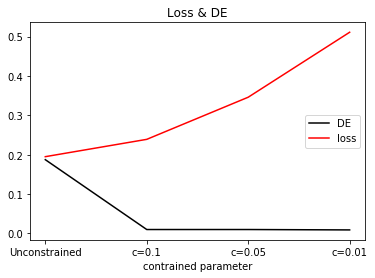
\includegraphics[height=3in]{logic_1.png}
    \caption{Logistic regression with constrained DE}
\end{figure}
\FloatBarrier
\hspace*{1em}We can also consider the decision boundary as expression for constraints. For linear classifier, the decision boundary equation can be reduced to $\theta^Tx=0$. 
In this case, the constraints are all linear. Then  it's a convex optimization problem:\\
The objective is:\\
\hspace*{12em}$\underset{\theta}{minimize} -\sum_{i=1}^{N}\,\,\, logp(y_i=1|x_i, \theta) \hfill(6)$\\
\hspace*{12em}subject to$ |A^T\theta|\leq c$(constrained on total variation)\\
\hspace*{1em}A: is a matrix with numbers of coefficients of xw, xz or zw.\\
\hspace*{1em}Lagrange multipliers can be employed here:\\
\centerline{$L(\theta,\lambda)=\,\,\,-\sum_{i=1}^{n}((y_i\theta x) -log(1+e^{\theta x}))+ \lambda_1(A^T\theta-c)+\lambda_2(-A^T\theta -c)$}
\hspace*{1em}Experiments: generate random data based on the causal model given before. $u_x, u_z, u_w, u_y$ are Bernoulli distributed with random parameter $p$ and the $f_x$, $f_z$, $f_w$,$f_y$ are defined according to the causal model we just referred at the beginning. \\
\hspace*{1em}Below is the constrained result for DE, IE, SE and total variation.\\
\\
\centerline{
 \begin{tabular}{c| c| c| c| c| c} 
 \hline
 & DE& IE & SE & TV & Loss  \\ [0.5ex] 
 \hline
Unconstrained & 0.3849& 0.2714 &  0.3508& 1.0071 &  0.0574\\ 
 \hline
Constrained(c=0.1) & -1.2702 & 0.2714 &  1.0780 &0.0792 & 0.3278 \\ [1ex] 
 \hline
 Constrained(c=0.05) & -1.3607 & 0.2714 &  1.1178 & 0.0285 & 0.3574 \\ [1ex] 
 \hline
 Constrained(c=0.01) & -1.4330 & 0.2714 &  1.1495 & -0.0121 & 0.3823 \\ [1ex] 
 \hline
\end{tabular}
}
\\
\FloatBarrier
\begin{figure}[!htb]
    \centering
    \subfloat[Loss and Total Variation]{{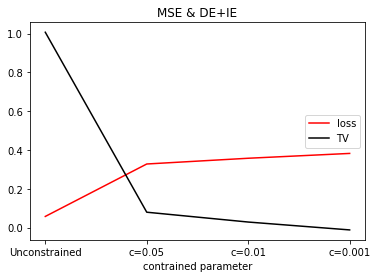
\includegraphics[height=2.3in]{logic_2.png} }}%
    \qquad
    \hspace*{-3em}
    \subfloat[DE, IE, SE, TV]{{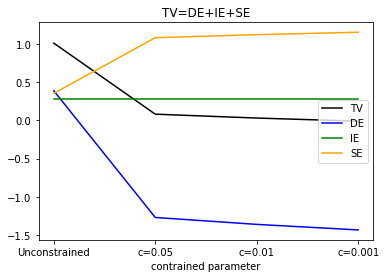
\includegraphics[height=2.3in]{logic_3.png} }}%
    \caption{logistic regression constrained on total variation}%
\end{figure}
\FloatBarrier
\hspace*{1em}From the plot we can see that as the total variation decreases, the loss increases. DE and SE increase to the inverse effect.\\
\hspace*{1em}Constrained on DE+IE:\\
\centerline{
 \begin{tabular}{c| c| c| c| c| c| c} 
 \hline
 & DE& IE & SE & TV&DE+IE & Loss  \\ [0.5ex] 
 \hline
Unconstrained & 0.3849& 0.2714 &  0.3508& 1.0071 &0.6563&  0.0574\\ 
 \hline
Constrained(c=0.1) & -0.1731 & 0.2731 &  0.6829 &0.7829&0.100 & 0.0735 \\ [1ex] 
 \hline
 Constrained(c=0.05) & -0.2232 & 0.2732 &  0.7127& 0.7627&0.050 & 0.0768 \\ [1ex] 
 \hline
 Constrained(c=0.01) & -0.2634 & 0.2734 &  0.7466 & 0.7466 &0.009& 0.0797 \\ [1ex] 
 \hline
\end{tabular}
}
\\
\FloatBarrier
\begin{figure}[!htb]
    \centering
    \subfloat[Loss and DE+IE]{{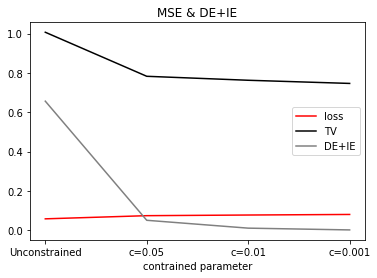
\includegraphics[height=2.3in]{logic_4.png} }}%
    \qquad
    \hspace*{-3em}
    \subfloat[DE, IE, SE, TV]{{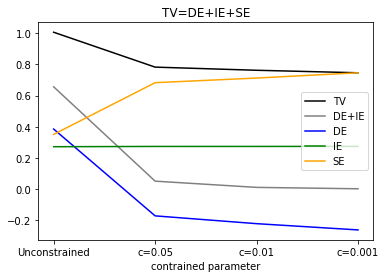
\includegraphics[height=2.3in]{logic_5.png} }}%
    \caption{logistic regression constrained on DE+IE}%
\end{figure}
\FloatBarrier
\hspace*{1em}From the above result, we can see that when constrained on DE+IE, the loss has a slightly increase.DE and total variation drops down. SE increases while IE keeps almost the same.\\
\hspace*{1em}Constrained on DE:\\
\\
\centerline{
 \begin{tabular}{c| c| c| c| c| c} 
 \hline
 & DE& IE & SE & TV & Loss  \\ [0.5ex] 
 \hline
Unconstrained & 0.3849& 0.2714 &  0.3508& 1.0071 &  0.0574\\ 
 \hline
Constrained(c=0.1) & 0.100 & 0.4429 &  0.4174 &0.9603 & 0.0588 \\ [1ex] 
 \hline
 Constrained(c=0.05) & 0.050 & 0.4730 &  0.4291 & 0.9521 & 0.0595 \\ [1ex] 
 \hline
 Constrained(c=0.01) & 0.0100 & 0.4971 &  0.4384& 0.9455 & 0.0602\\ [1ex] 
 \hline
\end{tabular}
}
\\
\FloatBarrier
\begin{figure}[!htb]
    \centering
    \subfloat[Loss and DE]{{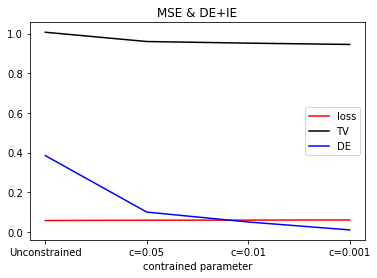
\includegraphics[height=2.3in]{logic_6.png} }}%
    \qquad
    \hspace*{-3em}
    \subfloat[DE, IE, SE, TV]{{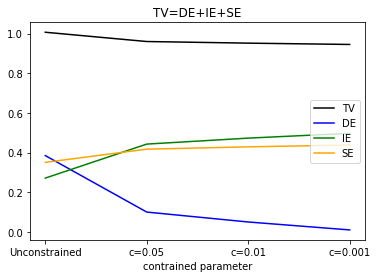
\includegraphics[height=2.3in]{logic_7.png} }}%
    \caption{logistic regression constrained on DE}%
\end{figure}
\FloatBarrier
\hspace*{1em}When constrained on DE, there is a trade-off between DE and loss. The total variation has a sightly decrease while IE and SE are all increasing.

\subsection{Fairness in Regression}
\hspace*{1em}We apply the causal fairness measures in linear regression models:\\
\hspace*{1em}Causal constraints: \\
\hspace*{5em}DE:  $DE_{x_0,x_1}(Y) = \beta_{xy}$,\\
\hspace*{5em}IE: $IE_{x_0,x_1}(Y) = \beta_{wy}\beta_{xw}$,\hfill(2)\\
\hspace*{5em}SE: $SE_{x_0,x_1}(Y) = (\beta_{zy}+\beta_{zw}\beta_{wy})\beta_{xz}$,\\
\hspace*{1em}Since we only care about the coefficients with respect to y, other coefficients can be considered as constants.\\
\hspace*{1em}which is : $|k_1\beta_{xy}+k_2\beta_{zy}+k_3\beta_{wy}|<c$(constrained on total variation)\\
\hspace*{1em}The boundary is convex with respect to coefficients $\beta$\\
\hspace*{1em}4. The whole problem can be written as:\\
\centerline{$\underset{\beta}{minimize}\,\,\,\sum_{i=1}^{n}(y_i-x_i^T\beta)^2$}
\centerline{subject to $k^T\beta\leq c, -k^T\beta\leq c$}
\hspace*{1em}The constraints can be written as Lagrange multipliers:\\
\centerline{$\underset{\beta}{minimize}\,\,\,\sum_{i=1}^{n}(y_i-x_i^T\beta)^2 + \lambda_1(k^T\beta-c)+\lambda_2(-k^T\beta -c)$}
\hspace*{1em}5.Experiments:\\
\hspace*{1em}Generate random data from standard normal distribution: $u_x, u_y, u_z, u_w$ are normally distributed. And also randomly select structural coefficients $\alpha$, $\theta$, $\gamma$ from standard normal distribution.\\
\hspace*{1em}Below is the discrimination after optimization compared to the discrimination measures without optimization:\\
\\
\centerline{
 \begin{tabular}{c| c| c| c| c| c} 
 \hline
 & DE& IE & SE & TV & MSE  \\ [0.5ex] 
 \hline
Unconstrained & 0.0600 & 0.1035 &  -0.5528& -0.3893 &  0.5358\\ 
 \hline
Constrained(c=0.1) & 0.3646 & 0.1035 &  -0.5164 &-0.0483 & 0.6703 \\ [1ex] 
 \hline
 Constrained(c=0.05) & 0.4088 & 0.1035 &  -0.5111 & 0.0012 & 0.7100 \\ [1ex] 
 \hline
 Constrained(c=0.001) & 0.4522 & 0.1035 &  -0.5060 & 0.0498 & 0.7538 \\ [1ex] 
 \hline
\end{tabular}
}
\\
\FloatBarrier
\begin{figure}[!htb]
    \centering
    \subfloat[MSE and Total Variation(absolute value)]{{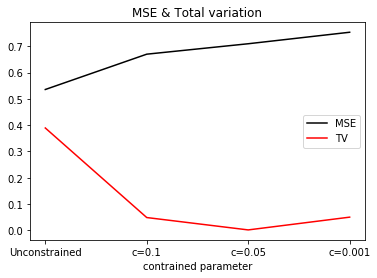
\includegraphics[height=2.3in]{regress_1.png} }}%
    \qquad
    \hspace*{-3em}
    \subfloat[DE, IE, SE, TV]{{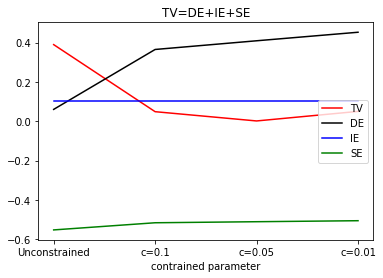
\includegraphics[height=2.3in]{regress_2.png} }}%
    \caption{linear regression constrained on total variation}%
\end{figure}
\FloatBarrier
\hspace*{1em}As we can see from the table, fairness constraints control the total variation by balancing the DE and SE while keeping IE almost the same. And the mean squared error is larger than the unconstrained case.\\
\\
\hspace*{1em}If we constrain on DE or DE+IE, below is the discrimination after optimization:\\
\centerline{
 \begin{tabular}{c| c| c| c| c| c} 
 \hline
 & DE& IE & SE & TV & MSE  \\ [0.5ex] 
 \hline
Unconstrained & 0.0600 & 0.1035 &  -0.5528& -0.3893 &  0.5358\\ 
 \hline
Constrained(c=0.05) &0.0500&0.1108&-0.5514&-0.3906&  0.5360 \\ [1ex] 
 \hline
 Constrained(c=0.01) & 0.0100 &0.1400&-0.5455&-0.3955& 0.5371 \\ [1ex] 
 \hline
 Constrained(c=0.001) & 9.9985e-04&0.1465&-0.5442&-0.3967 & 0.5374  \\ [1ex] 
 \hline
\end{tabular}
}
\\
\FloatBarrier
\begin{figure}[!htb]
    \centering
    \subfloat[MSE and DE]{{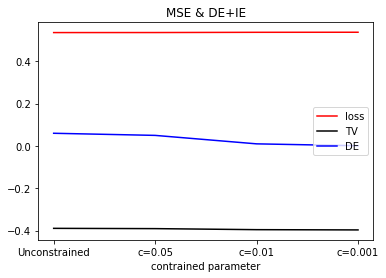
\includegraphics[height=2.3in]{regress_5.png} }}%
    \qquad
    \hspace*{-3em}
    \subfloat[DE, IE, SE, TV]{{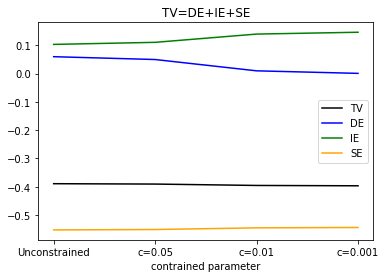
\includegraphics[height=2.3in]{regress_6.png} }}%
    \caption{linear regression constrained on DE}%
\end{figure}
\FloatBarrier
\hspace*{1em}When constrained on DE, the mean squared error seems to be the same. This because in this case the unconstrained direct counterfactual effect is small. The change of DE is very small to the whole model.\\
\\
\hspace*{1em}Constrained on DE+IE:\\
\\
\centerline{
 \begin{tabular}{c| c| c| c| c| c| c} 
 \hline
 & DE&IE&DE+IE&SE&TV& MSE  \\ [0.5ex] 
 \hline
Unconstrained & 0.0600&0.1035&0.1635  & -0.5528& -0.3893 &  0.5358\\ 
 \hline
Constrained(c=0.1) &0.0014& 0.0986&0.100&-0.5253&-0.4253&0.5345 \\ [1ex] 
 \hline
 Constrained(c=0.05) &-0.0447&0.0947&0.050&-0.5037&-0.4537&0.5360 \\ [1ex] 
 \hline
 Constrained(c=0.01) & -0.0816 & 0.0916&0.0100&-0.4864&-0.4764&0.5389 \\ [1ex] 
 \hline
\end{tabular}
}
\\
\FloatBarrier
\begin{figure}[!htb]
    \centering
    \subfloat[MSE and DE+IE]{{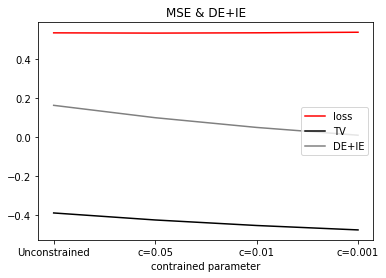
\includegraphics[height=2.3in]{regress_7.png} }}%
    \qquad
    \hspace*{-3em}
    \subfloat[DE, IE, SE, TV]{{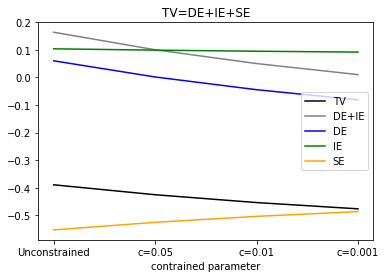
\includegraphics[height=2.3in]{regress_8.png} }}%
    \caption{linear regression constrained on DE+IE}%
\end{figure}
\FloatBarrier
\hspace*{1em}When constrained on DE+IE, DE decreases and then has reverse effect and IE keeps almost the same level. \\
\section{Conclusion}
\hspace*{2em}In conclusion,  our work firstly apply causal effect measures as constraints in decision making process. Binary domain is to maximize the likelihood with linear programming. In continuous domain, linear and convex utility maximization can be solved. Problems with special structural utilities can also be located to the global optimal solution. 
\\
\hspace*{1em}The future goal for this project is to apply the causal constraints to high dimensional data where things may be different. And also in nonlinear models the constraints are not linear with respect to regression coefficients. In addition, in many cases, the utility function is not well-defined or not deterministic. 


\section{Reference}
$[1]$ J. Zhang, E. Bareinboim. Fairness in Decision-Making -- The Causal Explanation Formula. AAAI-18. In Proceedings of the 32nd AAAI Conference on Artificial Intelligence, 2018, forthcoming. Purdue AI Lab, Technical Report (R-30), Nov, 2017.\\
$[2]$ S. C. Davies, E. Pierson, A. Feller. Algorithmic Decision Making and the Cost of Fairness, 2017\\
$[3]$ M. B. Zafar, I. Valera, M. G. Rodriguez, K. P. Gummadi. Fairness Constraints: Mechanisms for Fair Classification, 2017\\
$[4]$ M. Hardt, E. Price, N. Srebro. Equality of Opportunity in Supervised Learning, 2016\\
$[5]$ P. Hansen, B. Jaumard, S. H. Lu. Some Further Results on Monotonicity in Globally Optimal Design, 1989.\\
$[6]$ Alexander. Rubinov , Hoang. Tuy $\&$ Heather. Mays (2001) An alogrithm for monotonic global optimization problems , Optimization, 49:3, 205-221, DOI: 10.1080/02331930108844530\\


\end{document}
